\documentclass[conference]{IEEEtran}

% Packages for images, hyperlinks, and citations
\usepackage{graphicx}
\usepackage{amsmath}
\usepackage{hyperref}
\usepackage{cite}
\usepackage{amsfonts}
\usepackage{mathtools}

\usepackage{cleveref}
\crefname{figure}{Fig.}{Figs.} % Singular and plural formats

% Set bibliography style
\bibliographystyle{IEEEtran}

% For better font rendering
\usepackage[T1]{fontenc}
\usepackage{lmodern}
\usepackage[numbers]{natbib}

\begin{document}

\title{\bfseries Improving Computer Vision efficiency and inference performance through meta-understanding and cognitive robustness techniques in the real world }

\author{
    \IEEEauthorblockN{Sergio Gabardo}
    \IEEEauthorblockA{Pan American School of Porto Alegre \\
    2025sgabardo@panamerican.com.br}
}

\maketitle

\begin{abstract}
This research article, recognizing the exponentially-increasing power requirements large AI models are having in the last couple of years, provides a model-agnostic approach to increase model accuracy, reduce overfitting and training requirements via SAM, as well as prune model size and distillate knowledge to reduce overparameterization. These three main objectives highlight the approaches analyzed in this paper for a more efficient and lower-latency image classification high-dimentional ML model.
\end{abstract}

\IEEEpeerreviewmaketitle

\section{Introduction} \label{introduction}

\cite{aima2021} classifies the task of \textit{Artificial Intelligence} (AI) to ``build intelligent entities,'' emphasizing its ``truly universal field.'' \textit{Machine Learning} (ML), a subset of AI, leveraged by the power of \textit{Deep Learning} (DL), has seen astounding recent increases in influence, advancements, and general reach to the end consumers. Although current \textit{algorithms} and \textit{architectures} that of \textit{chatbots} or \textit{classification models}, when boiled down to their fundamentals, are not very different from that of past years, they have a giant distinction in how they are perceived and utilized by consumers. Take the \textit{Transformer} Architecture that powers modern chatbots: it was already 5 years old when first made available to the general public through \textit{ChatGPT} \cite{attention2017, chatgpt2022}.

\textit{Optical Character Recognition} (OCR) \cite{dtic1978}, which falls on the umbrella \textit{Computer Vision} (CV) field, widely utilized to convert images of car plates, printed numbers, or text into characters computers can interpret, has seen its first idealizations in the early 20th century (take Goldberg's 1927 \textit{Statistical Machine} \cite{goldberg1927}), with formal modern idealizations emerging later that same century \cite{hough1962, hough1962_patent}, streamlined by the widespread use of computers, digitalization of information, and implementations of new algorithms \cite{cnn1989, tesseract2006}. It becomes no doubt that, despite time passing by, advancements of ML, aiming to make computers as smart as possible \cite{aima2021}, are not a new technology per se, but rather ideas that are present in the idealizations of automation, intrinsic to human consciousness \cite{kahneman2011}.

This paper, henceforth, aims to analyze more efficient and accurate image-classification approaches in congruence with the recent astounding increase in energetical needs for training and running high-dimensional parameter spaces that of, but not limited to, \textit{Large Language Models} (LLMs) and \textit{Vision Transformers} (ViTs).

\subsection{How are models trained?}

A \textit{neural network} (NN) takes an input in the form of a \textit{feature vector}, which is fed into multiple \textit{neurons} which randomly activate based on the input. A model can be thought of as a black box analogy:
\begin{equation}
    \text{input} \to \boxed{\text{NN} } \to \text{output}
\end{equation}

The first step to understand how models succeed (or fail) to learn is to think of ML models the same way as we think of teaching others: we may not be aware of how they are reaching a conclusion, yet if they consistently reach one, it may be assumed their process is consistently reaching appropriate results (hence a low error or mistake rate). If students, however, consistently gets good grades in Test A, yet gets a statistically significant lower grade in Test B of the same content, it may be inferred that the student has not learned the actual content of the test, but rather its non-generalizable structure---this is called \textit{overfitting} in ML \cite{overfitting2004}. The notion of a student learning will henceforth be used, given the analogy's robustness and ability to capture well all the necessary concepts to be outlined in this paper. Training a ML algorithm, therefore, boils down to adapting teaching methods in order to conform to the best way students (models) learn.

Simplifying the calculation to a one-variable linear equation regression, there are two adjustable parameters: slope and $y$-intercept, and one output---the error. \cref{fig:training_evolution} demonstrates the evolution of a regression model as a ``descent'' into the valley. The valley in and of itself represents the optimal combination of parameters $m$ and $b$ to best fit the data.

\begin{figure}[htbp]
    \centering
    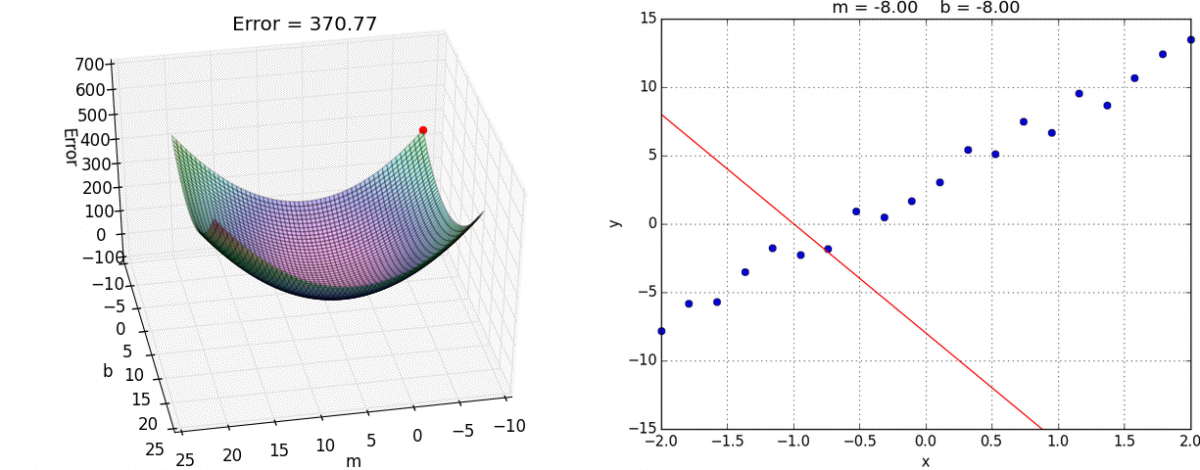
\includegraphics[width=0.45\textwidth]{images/frame_00_delay-0.2s.png}
    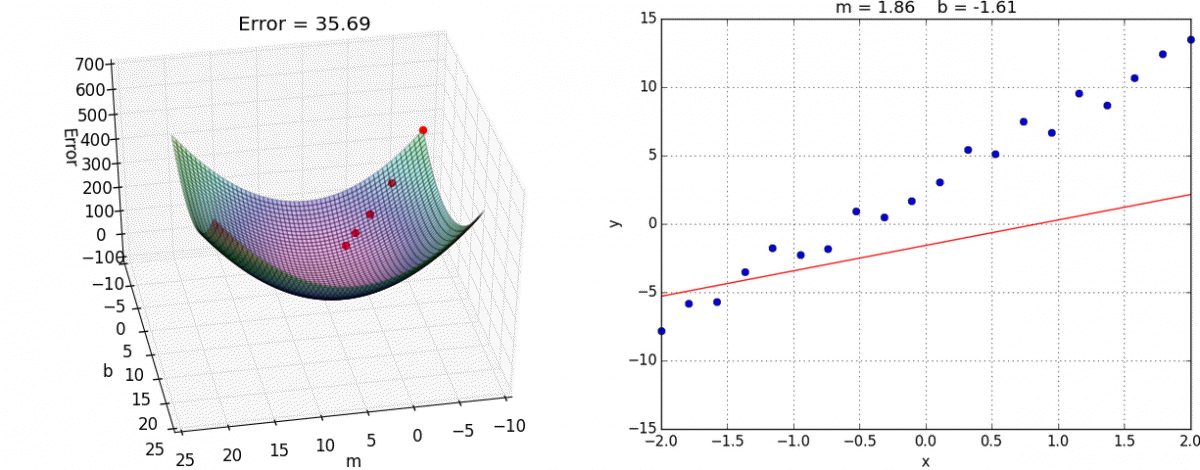
\includegraphics[width=0.45\textwidth]{images/frame_04_delay-0.2s.png}
    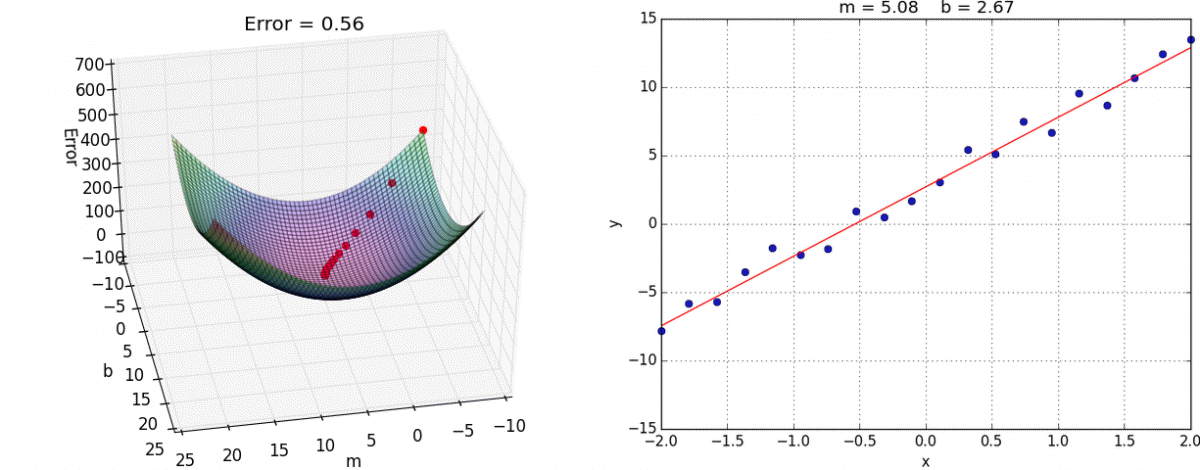
\includegraphics[width=0.45\textwidth]{images/frame_19_delay-0.2s.png}
    \caption{Visualization of error minimization: The loss landscape evolution (left) and corresponding best-fit line adjustments (right) demonstrate the iterative optimization process \cite{fig-yennhi95zz_evolution}.}
    \label{fig:training_evolution}
\end{figure}

There are some points that have to be cleared up prior to delving deeper, though: (i) this is a simplified model. It is clear to see what the answer is, but rather than two dimensions, current AI models such are already going into the trillions of parameters (i.e.\ dimensions); (ii) the error never, in a statistical scenario, reaches 0 due to sampling and data variability, and (iii) a valley may only be a \textit{local minima}, not necessarily the \textit{global} minima. The task in question is to minimize the chances of \textbf{not} reaching the optimal parameters.

With the scalar value from the \textit{objective function} (OF), one may understand that the focus is to minimize it. This is where backpropagation comes in. By analyzing how much changing one parameter affects it and its following neurons up to the final output layer through Calculus' \textit{Chain Rule}, a model is able to grasp how tuning different parameters evolves the \textbf{current model state} on the paraboloid shape provided by \cref{fig:training_evolution}'s loss lanscape, yet in a much higher-dimensional space.

It is additionally relevant to note that the evolution of the OF with respect to model training generally follows that of a decaying exponential function \eqref{eq:decay_function}

\begin{equation}
    f(n) = A\exp(-b\cdot n)+C, \quad A,\,b,\,C\in \mathbb{R}^+
    \label{eq:decay_function}
\end{equation}
where each value varies on a case-by-case basis depending on the evolution of the training and $n\in\mathbb{N}$ is the epoch number. $C$ is the \textit{steady state} (SS), that is, value the function approaches as $n\to \infty$. As the number of parameters of a function or regularization techniques applied increase, the SS tends to decrease given a better generalization over dataset $D$. However, every data set has an intrinsic entropy $H$, denoted $H(D)$ under the Shannon entropy formula \cite{shannon1948}.

The entropy of a dataset, often measured in bits per character (bpc), quantifies the average information content per character based on Shannon's formula \cite{shannon1961}. For example, the entropy of the whole English language, calculated in 1951, is c. 1 bpc as the number of characters $N\to \infty$. Howbeit, contingent on all 26 characters being randomly arranged in random order (remaining some arbitrary meaning), the average amount of information is of $\log_{2}(26)\approx 4.7$ bpc. This comes to show us that although different methods of conveying information exist, a pattern is always needed, typically in the form of data-loss protection. This explains why QR codes can function even with parts obscured, and why languages can omit certain words in sentences, yet both remain comprehensible to computers and humans.

The relevance of understanding both the general model evolution pattern and the entropy of a dataset is to firstly understand that, initially, models learn quickly yet begin to stall once finding smaller-error minima is harder than in the beginning. Moreover, the error of a non-overfit model can never be smaller than the intrinsic variability of the dataset itself. Note the last frame of \cref{fig:training_evolution}: neither is the best-fit line error or the MSE approaching zero, so much as they mathematically are not able to, at least with a line. The idea of the overparametrization of a dataset (as can be seen in \cref{fig:overfitting}) is a common issue in ML, which is be going to be further developed in section \ref{methodology}. If \cref{fig:training_evolution} was to approach a zero-error model, more parameters would have to be in play, but more would not represent a better generalization of the dataset.

\begin{figure}[htbp]
    \centering
    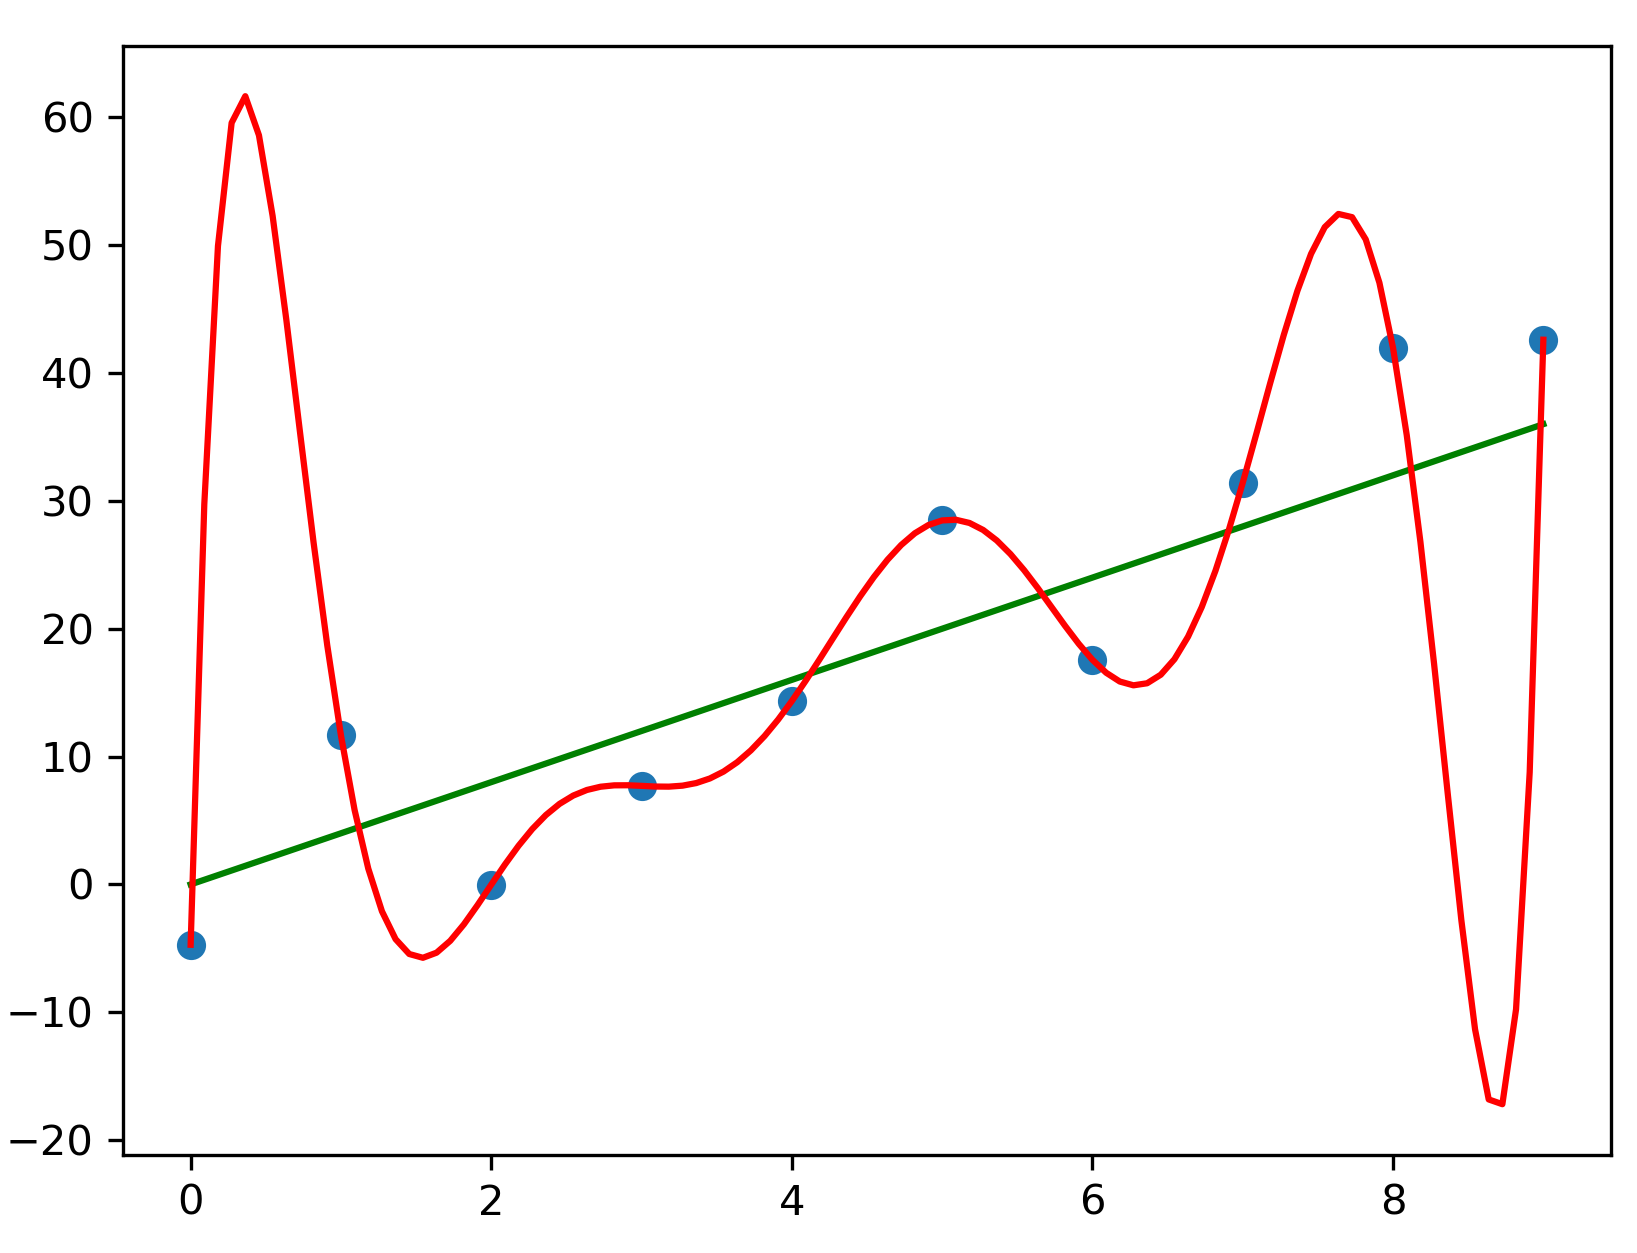
\includegraphics[width=0.45\textwidth]{images/overfitting.png}
    \caption{Illustration of overfitting: A high-degree polynomial (red) excessively conforms to a roughly linear dataset (blue), contrasting with the simpler best-fit linear model (green) \cite{fig-overfitting}.}
\label{fig:overfitting}
\end{figure}

\subsection{Backpropagation}
Although many of the training AI does is based on more complex and distinct processes than mere linear regression, the idea remains the same: we have a variable that measures by how off is a prediction, and we have to minimize it (hence the widespread use of $\displaystyle\min_{\theta}$ in many ML equations, where $\theta$ is the parameter to be minimized). The specific tuning of NNs is via a process called \textit{backpropagation}, where the \textit{gradient} (slope) of the loss function is used to calculate the \textit{vector field} (matching points of a graph with a vector) of the a function, such as that in \cref{fig:gradient_vectorfield}. This is the opposite process of \textit{forward propagation}: reaching conclusions given inputs.

\begin{figure}[htbp]
    \centering
    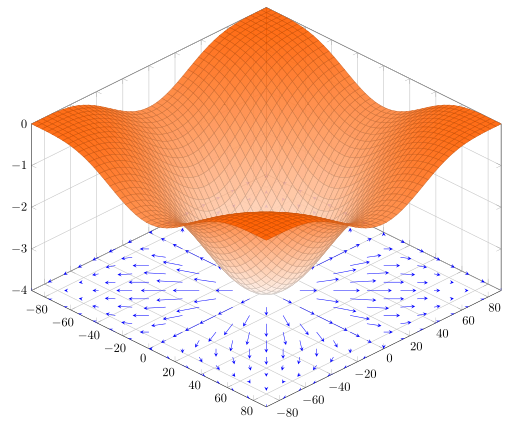
\includegraphics[width=0.45\textwidth]{images/3d-gradient-cos.png}
    \caption{Visualization of the gradient of the function $f(x, y) = -(\cos^2 x + \cos^2 y)^2$, showing the corresponding \textit{vector field} on the bottom plane. The arrows represent the gradient’s direction and magnitude, illustrating how the function’s slope guides optimization processes like backpropagation \cite{fig-gradient_vectorfield}.}
\label{fig:gradient_vectorfield}
\end{figure}

In simple terms, the gradient at any point in a function returns the vector of steepest ascent at any point. To reach local minima, consequently, we must take the negative gradient of the cost function at our current parameters, with the direction representing the parameters we have to change, and the magnitude by how much we must do so. The issues present with standard approaches to learning, together with ways of minimizing them are further detailed in section \ref{methodology}. A simplified formula \eqref{eq:sgd_formula} can be thought of as

\begin{equation}
    \theta_{t+1} = \theta_t - \eta \nabla_{\theta} \mathcal{L}(\theta_t)
    \label{eq:sgd_formula}
\end{equation}
where $\theta$ is the set of model parameters, $t$ is the epoch number (at what pass over the whole dataset the model is at), $\eta$ is the learning rate (also known as the step size), $\nabla_\theta$ is the gradient at the current parameters, and $\mathcal{L}$ is the loss function, taking the parameters as input. 

\section{Related Work} \label {related}

\subsection{Other methodologies employed}
All but one of the top 25 best image classifier models for at the CIFAR-100 dataset (90\% accuracy and up) showed use of ``extra training data'' \cite{SOTApwcIC}. Given the focus of this paper is to (i) provide means of reduced energy usage and (ii) improve robustness, this is a great source of information, notably due to the availability of thorough methodologies and code repositories.

\subsection{Other fields}

\subsubsection{Medical}
In a research experimentation with positive-negative pneumonia–classification cases in patients given x-ray photos, \cite{bundea2024} outlined a procedure similar to the objectives , with a model that (i) has small(er) size due to \textit{knowledge distillation}; (ii) general understanding with high accuracy due to being trained with a larger and more general dataset, (iii) avoiding the (a) \textbf{vanishing gradient}, (b) \textbf{unnecessarily rapid complexity growth}, and (c) \textbf{individual-neuron dependency} issues of traditional \textit{Convolutional Neural Networks} (CNNs), a specific type of NN used for image-classification tasks in the field of CV. In the methodology, the authors describe how all but the last hidden layers of the vanilla DenseNet model are frozen prior to fine tuning to a specific task. Besides reducing training needs, it avoids overfitting by maintaining better connections and stronger background prior to training and inference.

\subsubsection{Logistics}
In an optimization paper on one- and two-dimensional camera-interpreted machine-readable mediums, \cite{chen2024} demonstrated how the use of ML can consistently reduce the needs from human intervention or lack of information reading in situations where information matrices are partially hidden, skewed, or altered in some way such such that (i) accurate reading is more consistent among different tasks and (ii) reduces inference time and error rates.

\subsubsection{Robotics}
In a comparison between a rudimentary evolutionary and a state-of-the-art (SOTA) \textit{PPO} reinforcement learning (RL) ML model show that although for a much greater size, the better improved model has shown to have a much faster training performance despite significant additional resource requirements for a much better result in a shorter time \cite{RLsota2024}. Particularly for pre-trained models, they are extremely robust at what they do, and given that they have a strong meta-understanding of the general task, they are able to teach a smaller model in a much better way than any other model. The subfield of robotics, additionally, also includes autonomous driving vehicles, which by itself uses both RL and supervised-learning (SL) algorithms. Although significantly different, their ideas are similar, and both are going to be utilized on this research, notably for auto-hyperparameter tuning.

\subsection{Applications to this paper}
The three analyzed fields all greatly benefit from reductions in inference energy, time, and accuracy, without the overwhelming need of additional data for training, usually when additional training data (or occasions for RL applications) is typically too costly.
The solutions for these problems were highlighted in their respective papers. Each has their own strength, but the idea in this paper is to analyze how different methods combine within each other—to be further explained in the methodology section.

\section{Methodology} \label{methodology}

\subsection{What is the problem with standard methods?}

\subsubsection{Principle of least effort}
Traditional AI approaches, like standard \textit{Stochastic Gradient Descent} (SGD), simply move in the direction of the gradient, aiming to find a point of minimum energy. The issue is that with many parameters, as mentioned earlier, nearby local minima often aren't optimal in the parameter space, and hence, a model has to (i) repeat this process multiple times to make sure its specific points are even able to reach local minima, and (ii) initialize at multiple points to make sure of the full capturing of the loss function. Standard SGD would follow the same as \eqref{eq:sgd_formula}.

\subsubsection{Lack of meta-robustness}
Modern behavioral human minds think the way they do because of tens to hundreds of thousands of years of evolution and adaptation to our environment \cite{behavioral2007}. Although DL algorithms can simulate thousands to millions of years of evolution given enough computing power, it is clear that without proper guidance to help a model achieve human goals, no computer can achieve human-like performance. 

\subsubsection{Static model overparametrization}
A current issue in DL is that of \textit{scaling laws}, which empirically show how different model sizes, architectures, and training dataset sizes respond to distinct data inputs \cite{scaling_laws2020}. \cite{adaptive_model2024} provide a major change to standard \textit{static} models---that which have for the longest time been considered standard: \textit{adaptive} models. As much as model depth or width weakly correlate to model performance, ``performance depends strongly on scale'' \cite{scaling_laws2020}.

\subsection{Improved inference performance given improved training paradigms}

\subsubsection{Reasoning}
Evaluations show that, over the course of a model's lifecycle, approximately 10--20\% \cite{douwes2024} to 35\% \cite{sustainableAI2022} of its energy usage purely consists of training needs---with rest being solely used for inference up to the point where it is fully replaced by a newer model. It becomes clear, hence, that improving model inference performance is helpful as it leads to (i) improved results; (ii) better end-user satisfaction, and (iii) improved model turnover time (similar how employing better workers in a company leads to fewer future worker substitutions in a given time frame).

\subsubsection{Approach}
Rather than reducing training requirements, the presented rationale is to increase it. Instead of inefficiency, higher energy usages come as a result of higher robustness used for model preparation. The hypothesis is that by having a more robust way of reaching optimal parameters, a model will either (i) achieve a better final stable accuracy with similar number of parameters, or (ii) achieve similar metrics as traditional models with fewer parameters. In one hand, better accuracy leads to direct improvements without significant changes in the architecture, and in the other, smaller models lead to lower power draw. It is thought that, should these methods be implemented in a large---off-device---inference scale, the first alternative will be preferred. However, for small---on-device---inference, the second will be preferred.

\subsection{Course of action}

Several aforementioned hindrances to an ideal CV model have been identified. This section highlights the main points that will be utilized to counteract those points. 

\subsubsection{Sharpness-Aware Minimization}
Many examples one may encounter themselves with when searching the internet depict parameter spaces with clean, rounded, edges. Although it may be a misfortune for them not to be, \cite{sam2020}, demonstrate how a minimization technique proposed as \textit{Sharpness-Aware Minimization} (SAM), later expanded through Adaptive-SAM (ASAM) \cite{asam2021}, gets rid of jagged corners (refer to \cref{fig:sam} for a visualization). In this case, the principle of least effort (previously deemed as an innacuracy for regular models) has a higher chance of truly approaching a global minimum.

\begin{figure}[htbp]
    \centering
    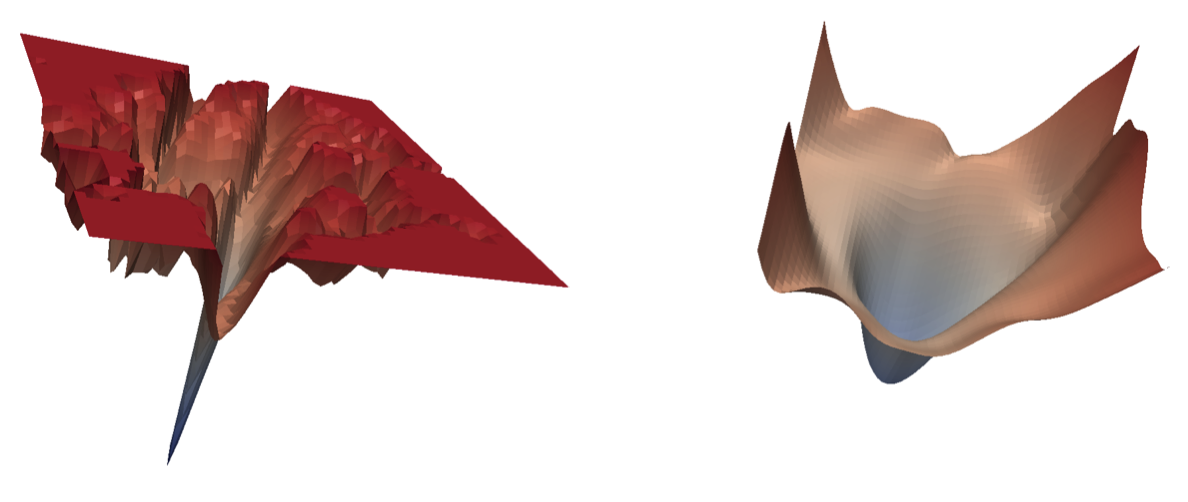
\includegraphics[width=0.45\textwidth]{images/sam.png}
    \caption{Comparison of parameter spaces: The original jagged parameter space (left) exhibits sharp and irregular contours, while the application of Sharpness-Aware Minimization (right) produces a smoother landscape, facilitating convergence toward a global minimum \cite{sam2020}.}
\label{fig:sam}
\end{figure}

\subsubsection{Robustness techniques}
In order to combat the typical lack of meta-robustness, two regularization approaches will be at play: the usage of \textit{Stochastic gradient Langevin dynamics} (SGLD) for the optimization technique, as well as \textit{data augmentation} (DA) of the dataset in question. SGLD helps, following the general idea previously provided at \eqref{eq:sgd_formula}, now with an additional layer of added \textit{Gaussian} noise. DA adds random crops, hue shifts in the color, flips, and so forth. The two techniques add to the dataset noise, seeking robustness future model inference. 

\subsubsection{Decreasing model size}
An adaptive-size model and random neuron dropout (ND) are the two techniques aiding the model from becoming too large or unnecessarily reliant on specific sections or neurons of the NN. While adaptive models have been previously discussed, ND has not. The process works by, during training, arbritrarily deactivating neurons. In turn, the model understand to distill knowledge among all of its neurons.

\subsection{Data preparation}

All analyses will be performed equally on all models, where the following are held constant among all models:

\begin{enumerate}
    \item Learning rate: $\eta=0.001$
    \item Activation function: ReLu\footnote{\textit{Rectified Linear Unit}, a popular NN activation function. $\text{ReLU}(\mathbf{z}) \coloneqq \max(0, \mathbf{z})$.}
    \item Loss function: Cross-entropy
    \item GPU: NVIDIA A100 80GB\footnote{Card will be run on \href{vast.ai}{\texttt{vast.ai}}, using the same provider for all runs for consistency.}
    \item Dataset: ImageNet and CIFAR-\{10, 100\}\footnote{Common image classification datasets consisting of thousands of images for both training and testing.}
\end{enumerate}

A couple parameters are relative to each configuration---following a general guide---such as the \textit{model stop}, which will depend on the average initial learning rate on that specific configuration.

All utilized code samples, datasets, additional remarks, further updates, and news are available in section \ref{resources}.

\subsection{Data analysis}
All data gotten from the models (final accuracy, scalar loss, epochs, power usage, etc.) can and will be used in order to determine to what extent the employment of different techniques were helpful, not helpful, or if they had no effect, and also to which extent they altered the final inference predictions of a model.

\section{Conclusion}

\subsection{Further explorations}
There are multiple considerations that have not been taking during this round of experimentation. The primary reason arises by the fact that CIFAR-\{10, 100\} is not a particularly diverse or complex dataset. The following explorations, although may be implemented in the same dataset, may not lead to significant improvements in performance given the truly greater increase in computational needs. In larger datasets, however, the implementation of the following could lead to improvements in most, if not all, of the aforementioned measured performance metrics.

\subsubsection{Combatting superlinear algorithmic performance growth through model modularization}

When inputting images to multimodal models of vertical text, rather than trying to flip the image (given much of the labeled data tend to in accordance with some basic assumptions that, for example, a user will only input data that makes sense to be read), the model will either (i) hallucinate into text that does not exist based on previous context or cues, or (ii) admit the text is not readable. Assumptions can also logically take place, such as in self-driving cars, which (hopefully) will not be looking at greatly rotated images. However, particularly in business-to-customer (B2C) interactions where coherence in the utilization of an interface is not always enforceable, having separate models with the sole job of making the raw data more easy to be interpreted by a pure classification model can greatly leverage both the performance of the classification and the reduction in computational needs due to the parsing of diverse data into ones that are consistent. The pipeline, or modular, architecture was not explored in this paper given both the complexity of the analysis dataset and the assumption is that the performance evaluations came after some level automated or human revision over the training data. Still, data augmentation was put in place in the assumption that revisions still left a margin of error comparable to that of the added variability.

Additionally, similar to the vertical information flow of the pipeline architecture, \textit{Mixture of Experts} (MoE) assimilates to an automated horizontal flow counterpart. The process is done during the training phase in a process analogous to that of \textit{unsupervised learning} (UL), where distinct inputs require distinct inference procedures, all of which that are clustered without the need of any labeled data. The hypothesis put forth is that MAML's quick adaptation, coupled with SGLD's high observability, have the potential to greatly improve MoE's expert selections. Better selection means each expert has to be less general to areas the automatic clustering process selected, leading to smaller, more efficient, models. Additionally, the paradigm has an astounding capability to reduce model utilization given that fractions of the whole model are to be called, instead of the total inference architecture.

\subsubsection{Combatting linearly proportional model growth}
Floating point constraints

Knowledge distillation: Models can get really large very quickly, yet this is not always beneficial, let alone efficient. Teacher-student in ML is a paradigm which makes a large model ``teach'' a smaller ``student'' model the intricacies of a task. This process can lead to substantially smaller models despite possessing similar performance levels.

\subsubsection{Additional variability}
Hyperparameters were chosen mainly on literary review and state-of-the-art models, not on empirical testing.

\section{Resources} \label{resources}

\subsection{Code samples}
All code utilized in this paper are available in \href{github.com}{this GitHub repo}.\footnote{Not yet available as of yet.}

\subsection{Further reading}

\begin{enumerate}
    \item \href{https://interactive-maml.github.io/}{Interactive MAML} \cite{interactive_maml}
    \item \href{https://youtube.com/playlist?list=PLZHQObOWTQDNU6R1_67000Dx_ZCJB-3pi}{Neural networks} \cite{3b1b_nn}
\end{enumerate}

\bibliography{CV_Efficiency_MetaRobustness}

\end{document}